\documentclass[]{article}
\usepackage{lmodern}
\usepackage{amssymb,amsmath}
\usepackage{ifxetex,ifluatex}
\usepackage{fixltx2e} % provides \textsubscript
\ifnum 0\ifxetex 1\fi\ifluatex 1\fi=0 % if pdftex
  \usepackage[T1]{fontenc}
  \usepackage[utf8]{inputenc}
\else % if luatex or xelatex
  \ifxetex
    \usepackage{mathspec}
  \else
    \usepackage{fontspec}
  \fi
  \defaultfontfeatures{Ligatures=TeX,Scale=MatchLowercase}
\fi
% use upquote if available, for straight quotes in verbatim environments
\IfFileExists{upquote.sty}{\usepackage{upquote}}{}
% use microtype if available
\IfFileExists{microtype.sty}{%
\usepackage{microtype}
\UseMicrotypeSet[protrusion]{basicmath} % disable protrusion for tt fonts
}{}
\usepackage[margin=1in]{geometry}
\usepackage{hyperref}
\hypersetup{unicode=true,
            pdftitle={Activity Monitoring Analysis},
            pdfauthor={Aliakbar Safilian},
            pdfborder={0 0 0},
            breaklinks=true}
\urlstyle{same}  % don't use monospace font for urls
\usepackage{color}
\usepackage{fancyvrb}
\newcommand{\VerbBar}{|}
\newcommand{\VERB}{\Verb[commandchars=\\\{\}]}
\DefineVerbatimEnvironment{Highlighting}{Verbatim}{commandchars=\\\{\}}
% Add ',fontsize=\small' for more characters per line
\usepackage{framed}
\definecolor{shadecolor}{RGB}{248,248,248}
\newenvironment{Shaded}{\begin{snugshade}}{\end{snugshade}}
\newcommand{\KeywordTok}[1]{\textcolor[rgb]{0.13,0.29,0.53}{\textbf{#1}}}
\newcommand{\DataTypeTok}[1]{\textcolor[rgb]{0.13,0.29,0.53}{#1}}
\newcommand{\DecValTok}[1]{\textcolor[rgb]{0.00,0.00,0.81}{#1}}
\newcommand{\BaseNTok}[1]{\textcolor[rgb]{0.00,0.00,0.81}{#1}}
\newcommand{\FloatTok}[1]{\textcolor[rgb]{0.00,0.00,0.81}{#1}}
\newcommand{\ConstantTok}[1]{\textcolor[rgb]{0.00,0.00,0.00}{#1}}
\newcommand{\CharTok}[1]{\textcolor[rgb]{0.31,0.60,0.02}{#1}}
\newcommand{\SpecialCharTok}[1]{\textcolor[rgb]{0.00,0.00,0.00}{#1}}
\newcommand{\StringTok}[1]{\textcolor[rgb]{0.31,0.60,0.02}{#1}}
\newcommand{\VerbatimStringTok}[1]{\textcolor[rgb]{0.31,0.60,0.02}{#1}}
\newcommand{\SpecialStringTok}[1]{\textcolor[rgb]{0.31,0.60,0.02}{#1}}
\newcommand{\ImportTok}[1]{#1}
\newcommand{\CommentTok}[1]{\textcolor[rgb]{0.56,0.35,0.01}{\textit{#1}}}
\newcommand{\DocumentationTok}[1]{\textcolor[rgb]{0.56,0.35,0.01}{\textbf{\textit{#1}}}}
\newcommand{\AnnotationTok}[1]{\textcolor[rgb]{0.56,0.35,0.01}{\textbf{\textit{#1}}}}
\newcommand{\CommentVarTok}[1]{\textcolor[rgb]{0.56,0.35,0.01}{\textbf{\textit{#1}}}}
\newcommand{\OtherTok}[1]{\textcolor[rgb]{0.56,0.35,0.01}{#1}}
\newcommand{\FunctionTok}[1]{\textcolor[rgb]{0.00,0.00,0.00}{#1}}
\newcommand{\VariableTok}[1]{\textcolor[rgb]{0.00,0.00,0.00}{#1}}
\newcommand{\ControlFlowTok}[1]{\textcolor[rgb]{0.13,0.29,0.53}{\textbf{#1}}}
\newcommand{\OperatorTok}[1]{\textcolor[rgb]{0.81,0.36,0.00}{\textbf{#1}}}
\newcommand{\BuiltInTok}[1]{#1}
\newcommand{\ExtensionTok}[1]{#1}
\newcommand{\PreprocessorTok}[1]{\textcolor[rgb]{0.56,0.35,0.01}{\textit{#1}}}
\newcommand{\AttributeTok}[1]{\textcolor[rgb]{0.77,0.63,0.00}{#1}}
\newcommand{\RegionMarkerTok}[1]{#1}
\newcommand{\InformationTok}[1]{\textcolor[rgb]{0.56,0.35,0.01}{\textbf{\textit{#1}}}}
\newcommand{\WarningTok}[1]{\textcolor[rgb]{0.56,0.35,0.01}{\textbf{\textit{#1}}}}
\newcommand{\AlertTok}[1]{\textcolor[rgb]{0.94,0.16,0.16}{#1}}
\newcommand{\ErrorTok}[1]{\textcolor[rgb]{0.64,0.00,0.00}{\textbf{#1}}}
\newcommand{\NormalTok}[1]{#1}
\usepackage{graphicx,grffile}
\makeatletter
\def\maxwidth{\ifdim\Gin@nat@width>\linewidth\linewidth\else\Gin@nat@width\fi}
\def\maxheight{\ifdim\Gin@nat@height>\textheight\textheight\else\Gin@nat@height\fi}
\makeatother
% Scale images if necessary, so that they will not overflow the page
% margins by default, and it is still possible to overwrite the defaults
% using explicit options in \includegraphics[width, height, ...]{}
\setkeys{Gin}{width=\maxwidth,height=\maxheight,keepaspectratio}
\IfFileExists{parskip.sty}{%
\usepackage{parskip}
}{% else
\setlength{\parindent}{0pt}
\setlength{\parskip}{6pt plus 2pt minus 1pt}
}
\setlength{\emergencystretch}{3em}  % prevent overfull lines
\providecommand{\tightlist}{%
  \setlength{\itemsep}{0pt}\setlength{\parskip}{0pt}}
\setcounter{secnumdepth}{0}
% Redefines (sub)paragraphs to behave more like sections
\ifx\paragraph\undefined\else
\let\oldparagraph\paragraph
\renewcommand{\paragraph}[1]{\oldparagraph{#1}\mbox{}}
\fi
\ifx\subparagraph\undefined\else
\let\oldsubparagraph\subparagraph
\renewcommand{\subparagraph}[1]{\oldsubparagraph{#1}\mbox{}}
\fi

%%% Use protect on footnotes to avoid problems with footnotes in titles
\let\rmarkdownfootnote\footnote%
\def\footnote{\protect\rmarkdownfootnote}

%%% Change title format to be more compact
\usepackage{titling}

% Create subtitle command for use in maketitle
\newcommand{\subtitle}[1]{
  \posttitle{
    \begin{center}\large#1\end{center}
    }
}

\setlength{\droptitle}{-2em}

  \title{Activity Monitoring Analysis}
    \pretitle{\vspace{\droptitle}\centering\huge}
  \posttitle{\par}
    \author{Aliakbar Safilian\footnote{\href{mailto:a.a.safilian@gmail.com}{\nolinkurl{a.a.safilian@gmail.com}}}}
    \preauthor{\centering\large\emph}
  \postauthor{\par}
      \predate{\centering\large\emph}
  \postdate{\par}
    \date{October 2018}


\begin{document}
\maketitle

\subsection{Overview}\label{overview}

This project makes use of data from a personal activity monitoring
device. This device collects data at 5 minute intervals through out the
day. The data consists of two months of data from an anonymous
individual collected during the months of October and November, 2012 and
include the number of steps taken in 5 minute intervals each day.

The data for this assignment can be downloaded from
\url{https://d396qusza40orc.cloudfront.net/repdata\%2Fdata\%2Factivity.zip}.

The variables included in this dataset are:

\begin{itemize}
\tightlist
\item
  steps: Number of steps taking in a 5-minute interval\\
\item
  date: The date on which the measurement was taken in YYYY-MM-DD format
\item
  interval: Identifier for the 5-minute interval in which measurement
  was taken
\end{itemize}

There are a total of 17,568 observations in this dataset.

We need to load the following libraries:

\begin{Shaded}
\begin{Highlighting}[]
\KeywordTok{library}\NormalTok{(dplyr)}
\KeywordTok{library}\NormalTok{(chron)}
\KeywordTok{library}\NormalTok{(lattice)}
\KeywordTok{library}\NormalTok{(ggplot2)}
\end{Highlighting}
\end{Shaded}

\subsection{Loading and preprocessing the
data}\label{loading-and-preprocessing-the-data}

In the following script, we load the data using by the \emph{read.csv}
and the \emph{unzip} functions, and save it into a variable called
\textbf{data}. The zip file (``activity.zip'') is already in the repo.

\begin{Shaded}
\begin{Highlighting}[]
\NormalTok{data <-}\StringTok{ }\KeywordTok{read.csv}\NormalTok{(}\KeywordTok{unzip}\NormalTok{(}\StringTok{"activity.zip"}\NormalTok{, }\StringTok{"activity.csv"}\NormalTok{))}
\KeywordTok{str}\NormalTok{(data)}
\end{Highlighting}
\end{Shaded}

\begin{verbatim}
## 'data.frame':    17568 obs. of  3 variables:
##  $ steps   : int  NA NA NA NA NA NA NA NA NA NA ...
##  $ date    : Factor w/ 61 levels "2012-10-01","2012-10-02",..: 1 1 1 1 1 1 1 1 1 1 ...
##  $ interval: int  0 5 10 15 20 25 30 35 40 45 ...
\end{verbatim}

As we see, the \textbf{date} variable is a factor. In the follwoing
script, we transform it to a \emph{Date} variable.

\begin{Shaded}
\begin{Highlighting}[]
\NormalTok{data <-}\StringTok{ }\KeywordTok{transform}\NormalTok{(data, }\DataTypeTok{date =} \KeywordTok{as.Date}\NormalTok{(date))}
\KeywordTok{str}\NormalTok{(data)}
\end{Highlighting}
\end{Shaded}

\begin{verbatim}
## 'data.frame':    17568 obs. of  3 variables:
##  $ steps   : int  NA NA NA NA NA NA NA NA NA NA ...
##  $ date    : Date, format: "2012-10-01" "2012-10-01" ...
##  $ interval: int  0 5 10 15 20 25 30 35 40 45 ...
\end{verbatim}

Before going to the next step, let us see how many of the observations
got missing values for each variables.

\begin{Shaded}
\begin{Highlighting}[]
\NormalTok{stepsNA <-}\StringTok{ }\KeywordTok{mean}\NormalTok{(}\KeywordTok{is.na}\NormalTok{(data}\OperatorTok{$}\NormalTok{steps)) }\OperatorTok{*}\DecValTok{100}
\NormalTok{dateNA <-}\StringTok{ }\KeywordTok{mean}\NormalTok{(}\KeywordTok{is.na}\NormalTok{(data}\OperatorTok{$}\NormalTok{date)) }\OperatorTok{*}\DecValTok{100}
\NormalTok{intervalNA <-}\StringTok{ }\KeywordTok{mean}\NormalTok{(}\KeywordTok{is.na}\NormalTok{(data}\OperatorTok{$}\NormalTok{interval)) }\OperatorTok{*}\DecValTok{100}
\end{Highlighting}
\end{Shaded}

So, the proportion of NA values w.r.t the whole data in \textbf{steps},
\textbf{date}, and \textbf{interval} are 13\%, 0\%, and 0\%,
respectively.

\section{What is mean total number of steps taken per
day?}\label{what-is-mean-total-number-of-steps-taken-per-day}

We get ``\emph{the total number of steps taken per day}'' by the
following script.

\begin{Shaded}
\begin{Highlighting}[]
\NormalTok{stepsday <-}\StringTok{ }\NormalTok{data }\OperatorTok\StringTok{ }\KeywordTok{group_by}\NormalTok{(date) }\OperatorTok\StringTok{ }\KeywordTok{summarize}\NormalTok{(}\DataTypeTok{totalSteps =} \KeywordTok{sum}\NormalTok{(steps, }\DataTypeTok{na.rm =} \OtherTok{TRUE}\NormalTok{))}
\NormalTok{stepsday}
\end{Highlighting}
\end{Shaded}

\begin{verbatim}
## # A tibble: 61 x 2
##    date       totalSteps
##    <date>          <int>
##  1 2012-10-01          0
##  2 2012-10-02        126
##  3 2012-10-03      11352
##  4 2012-10-04      12116
##  5 2012-10-05      13294
##  6 2012-10-06      15420
##  7 2012-10-07      11015
##  8 2012-10-08          0
##  9 2012-10-09      12811
## 10 2012-10-10       9900
## # ... with 51 more rows
\end{verbatim}

Here is the ``\emph{histogram of the total number of steps taken each
day}'':

\begin{Shaded}
\begin{Highlighting}[]
\KeywordTok{hist}\NormalTok{(stepsday}\OperatorTok{$}\NormalTok{totalSteps, }\DataTypeTok{col =} \StringTok{"green"}\NormalTok{, }\DataTypeTok{breaks =} \DecValTok{7}\NormalTok{, }\DataTypeTok{main =} \StringTok{"Histogram of number of steps taken each day"}\NormalTok{, }\DataTypeTok{xlab =} \StringTok{"Total Steps"}\NormalTok{)}
\KeywordTok{rug}\NormalTok{(stepsday}\OperatorTok{$}\NormalTok{totalSteps) }
\KeywordTok{abline}\NormalTok{(}\DataTypeTok{v =} \KeywordTok{median}\NormalTok{(stepsday}\OperatorTok{$}\NormalTok{totalSteps, }\DataTypeTok{na.rm =}\NormalTok{ T), }\DataTypeTok{col =} \StringTok{"magenta"}\NormalTok{, }\DataTypeTok{lwd =} \DecValTok{4}\NormalTok{)}
\KeywordTok{abline}\NormalTok{(}\DataTypeTok{v =} \KeywordTok{mean}\NormalTok{(stepsday}\OperatorTok{$}\NormalTok{totalSteps, }\DataTypeTok{na.rm =}\NormalTok{ T), }\DataTypeTok{lwd =} \DecValTok{4}\NormalTok{)}
\end{Highlighting}
\end{Shaded}

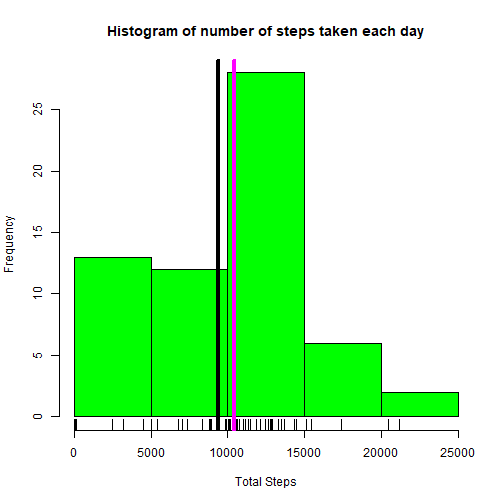
\includegraphics{PA1_template_files/figure-latex/histogram-steps-1.pdf}

In the following script, we calculate the ``\emph{mean and median of the
total number of steps taken per day}''.

\begin{Shaded}
\begin{Highlighting}[]
\NormalTok{stepsmean <-}\StringTok{ }\KeywordTok{mean}\NormalTok{(stepsday}\OperatorTok{$}\NormalTok{totalSteps)}
\NormalTok{stepsmedian <-}\StringTok{ }\KeywordTok{median}\NormalTok{(stepsday}\OperatorTok{$}\NormalTok{totalSteps)}
\end{Highlighting}
\end{Shaded}

The mean and median of total number of steps taken per day are
\textbf{9354.2295082} and \textbf{10395}, respecitvely. The megenta and
black vertical lines in the above histogram show them, respectively.

\subsection{What is the average daily activity
pattern?}\label{what-is-the-average-daily-activity-pattern}

The following script calculates the average number of steps, averaged
across all days per interval. The result is shown in a plot.

\begin{Shaded}
\begin{Highlighting}[]
\NormalTok{avgstpinv <-}\StringTok{ }\NormalTok{data }\OperatorTok\StringTok{ }\KeywordTok{group_by}\NormalTok{(interval) }\OperatorTok\StringTok{ }\KeywordTok{summarize}\NormalTok{(}\DataTypeTok{avgerage_steps =} \KeywordTok{mean}\NormalTok{(steps, }\DataTypeTok{na.rm =} \OtherTok{TRUE}\NormalTok{))}
\KeywordTok{plot}\NormalTok{(avgstpinv, }\DataTypeTok{type =} \StringTok{"l"}\NormalTok{, }\DataTypeTok{main =} \StringTok{"Average Steps per Interval"}\NormalTok{)}
\end{Highlighting}
\end{Shaded}

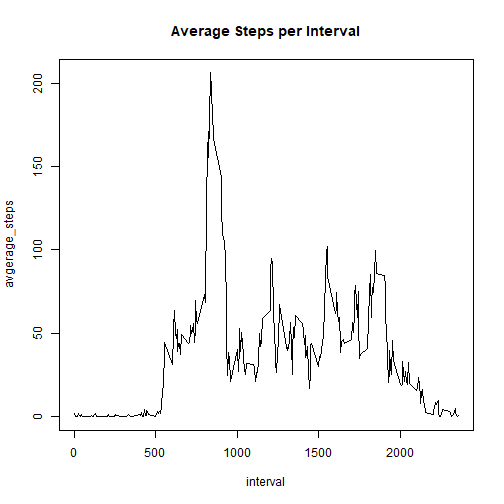
\includegraphics{PA1_template_files/figure-latex/avg-stp-inv-1.pdf}

The following script gets the interval, which contains the maximum
number of steps, averaged across all the days.

\begin{Shaded}
\begin{Highlighting}[]
\NormalTok{maxinvstp <-}\StringTok{ }\NormalTok{avgstpinv}\OperatorTok{$}\NormalTok{interval[}\KeywordTok{which}\NormalTok{(avgstpinv}\OperatorTok{$}\NormalTok{avgerage_steps }\OperatorTok{==}\StringTok{ }\KeywordTok{max}\NormalTok{(avgstpinv}\OperatorTok{$}\NormalTok{avgerage_steps))]}
\end{Highlighting}
\end{Shaded}

So, the interval, which contains the maximum number of average steps is
\textbf{835}.

\subsection{Imputing missing values}\label{imputing-missing-values}

The total number of \textbf{NA} rows in \textbf{data} is calculated as
follows:

\begin{Shaded}
\begin{Highlighting}[]
\NormalTok{nanum <-}\StringTok{ }\KeywordTok{sum}\NormalTok{(}\KeywordTok{is.na}\NormalTok{(data))}
\NormalTok{nanum}
\end{Highlighting}
\end{Shaded}

\begin{verbatim}
## [1] 2304
\end{verbatim}

The following script replaces the \textbf{NA} values in \textbf{steps}
with the mean of all \textbf{steps} taken in the corresponding interval.
We take advantage of the data frame created in the former stages.

\begin{Shaded}
\begin{Highlighting}[]
\ControlFlowTok{for}\NormalTok{(i }\ControlFlowTok{in} \DecValTok{1}\OperatorTok{:}\KeywordTok{dim}\NormalTok{(data)[}\DecValTok{1}\NormalTok{])\{}
        \ControlFlowTok{if}\NormalTok{(}\KeywordTok{is.na}\NormalTok{(data}\OperatorTok{$}\NormalTok{steps)[i])\{}
\NormalTok{                data}\OperatorTok{$}\NormalTok{steps[i] <-}\StringTok{ }\NormalTok{avgstpinv[avgstpinv}\OperatorTok{$}\NormalTok{interval }\OperatorTok{==}\StringTok{ }\NormalTok{data}\OperatorTok{$}\NormalTok{interval[i],]}\OperatorTok{$}\NormalTok{avgerage_steps}
\NormalTok{        \}}
\NormalTok{\}}
\end{Highlighting}
\end{Shaded}

As we see now, in the following script, there is no missing values in
our data anymore.

\begin{Shaded}
\begin{Highlighting}[]
\KeywordTok{sum}\NormalTok{(}\KeywordTok{is.na}\NormalTok{(data))}
\end{Highlighting}
\end{Shaded}

\begin{verbatim}
## [1] 0
\end{verbatim}

Now, here is the updated ``\emph{histogram of the total number of steps
taken each day}''. We first get the total number of steps taken per day
and store the data in a data frame named \textbf{stepsday2}.

\begin{Shaded}
\begin{Highlighting}[]
\NormalTok{stepsday2 <-}\StringTok{ }\NormalTok{data }\OperatorTok\StringTok{ }\KeywordTok{group_by}\NormalTok{(date) }\OperatorTok\StringTok{ }\KeywordTok{summarize}\NormalTok{(}\DataTypeTok{totalSteps =} \KeywordTok{sum}\NormalTok{(steps, }\DataTypeTok{na.rm =}\NormalTok{ T))}

\KeywordTok{hist}\NormalTok{(stepsday2}\OperatorTok{$}\NormalTok{totalSteps, }\DataTypeTok{col =} \StringTok{"green"}\NormalTok{, }\DataTypeTok{main =} \StringTok{"Histogram of number of steps taken each day"}\NormalTok{, }\DataTypeTok{xlab =} \StringTok{"Total Steps"}\NormalTok{)}
\KeywordTok{rug}\NormalTok{(stepsday2}\OperatorTok{$}\NormalTok{totalSteps) }
\KeywordTok{abline}\NormalTok{(}\DataTypeTok{v =} \KeywordTok{median}\NormalTok{(stepsday2}\OperatorTok{$}\NormalTok{totalSteps), }\DataTypeTok{col =} \StringTok{"magenta"}\NormalTok{, }\DataTypeTok{lwd =} \DecValTok{2}\NormalTok{, }\DataTypeTok{lty =} \DecValTok{2}\NormalTok{)}
\end{Highlighting}
\end{Shaded}

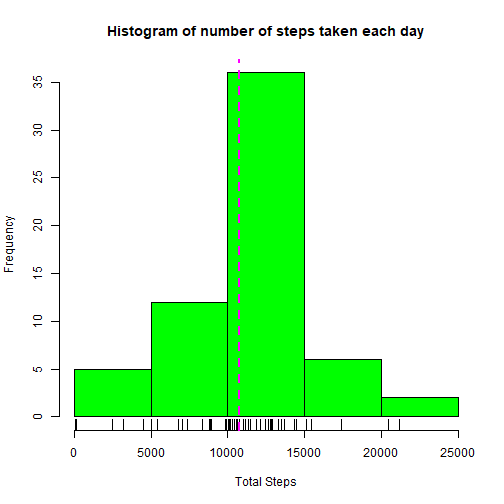
\includegraphics{PA1_template_files/figure-latex/histogram-steps-updated-1.pdf}

\begin{Shaded}
\begin{Highlighting}[]
\CommentTok{#abline(v = mean(stepsday2$totalSteps), lwd = 2)}
\NormalTok{meann <-}\StringTok{ }\KeywordTok{mean}\NormalTok{(stepsday2}\OperatorTok{$}\NormalTok{totalSteps)}
\NormalTok{mediann <-}\KeywordTok{median}\NormalTok{(stepsday2}\OperatorTok{$}\NormalTok{totalSteps)}
\end{Highlighting}
\end{Shaded}

As we see in the plot, the median and mean of the total steps per day
are now eqaul: mean == 1.0766189\times 10\^{}\{4\} == median.

\subsection{Are there differences in activity patterns between weekdays
and
weekends?}\label{are-there-differences-in-activity-patterns-between-weekdays-and-weekends}

In the following script, we create a factor variable, named
\textbf{wday} in \textbf{data} with two levels -- ``weekday'' and
``weekend''-- indicating whether a given date is a weekday or weekend
day.

\begin{Shaded}
\begin{Highlighting}[]
\NormalTok{data}\OperatorTok{$}\NormalTok{wdays <-}\StringTok{ }\KeywordTok{weekdays}\NormalTok{(data}\OperatorTok{$}\NormalTok{date)}
\ControlFlowTok{for}\NormalTok{(i }\ControlFlowTok{in} \DecValTok{1}\OperatorTok{:}\KeywordTok{dim}\NormalTok{(data)[}\DecValTok{1}\NormalTok{])\{}
        \ControlFlowTok{if}\NormalTok{(data}\OperatorTok{$}\NormalTok{wdays[i] }\OperatorTok{==}\StringTok{ "Saturday"} \OperatorTok{|}\StringTok{ }\NormalTok{data}\OperatorTok{$}\NormalTok{wdays[i] }\OperatorTok{==}\StringTok{ "Sunday"}\NormalTok{) \{}
\NormalTok{                data}\OperatorTok{$}\NormalTok{wdays[i] <-}\StringTok{ "weekend"}
\NormalTok{        \}}
        \ControlFlowTok{else}\NormalTok{\{}
\NormalTok{                data}\OperatorTok{$}\NormalTok{wdays[i] <-}\StringTok{ "weekday"}
\NormalTok{        \}}
\NormalTok{\}}
\NormalTok{data}\OperatorTok{$}\NormalTok{wdays <-}\StringTok{ }\KeywordTok{as.factor}\NormalTok{(data}\OperatorTok{$}\NormalTok{wdays)}
\end{Highlighting}
\end{Shaded}

Now, in the following script, we make a panel plot containing a time
series plot of the interval (x-axis) and the average number of steps
taken, averaged across all weekday days or weekend days (y-axis).

\begin{Shaded}
\begin{Highlighting}[]
\NormalTok{avgstp <-}\StringTok{ }\NormalTok{data }\OperatorTok\StringTok{ }\KeywordTok{group_by}\NormalTok{(wdays, interval) }\OperatorTok\StringTok{ }\KeywordTok{summarize}\NormalTok{(}\DataTypeTok{avg_steps =} \KeywordTok{mean}\NormalTok{(steps, }\DataTypeTok{na.rm =} \OtherTok{TRUE}\NormalTok{))}
\KeywordTok{xyplot}\NormalTok{(avg_steps }\OperatorTok{~}\StringTok{ }\NormalTok{interval }\OperatorTok{|}\StringTok{ }\NormalTok{wdays, }\DataTypeTok{data =}\NormalTok{ avgstp,  }\DataTypeTok{type =} \StringTok{"l"}\NormalTok{, }\DataTypeTok{ylab =} \StringTok{"Number of steps"}\NormalTok{, }\DataTypeTok{main =} \StringTok{"Average number of Steps per interval"}\NormalTok{)}
\end{Highlighting}
\end{Shaded}

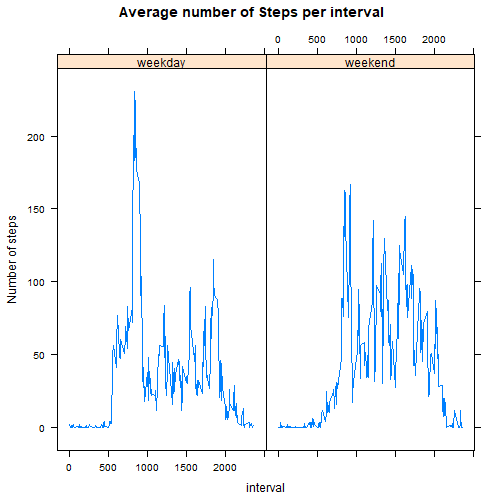
\includegraphics{PA1_template_files/figure-latex/unnamed-chunk-3-1.pdf}


\end{document}
